\chapter{Árvores de segmentos revisitadas}

\index{árvore de segmentos}

Uma árvore de segmentos é uma estrutura de dados versátil que pode ser usada para resolver um grande número de problemas algorítmicos. No entanto, há muitos tópicos relacionados a árvores de segmentos que ainda não abordamos. Agora é hora de discutir algumas variantes mais avançadas de árvores de segmentos.

Até agora, implementamos as operações de uma árvore de segmentos percorrendo \emph{de baixo para cima} na árvore. Por exemplo, calculamos somas de intervalo da seguinte forma (Capítulo 9.3):

\begin{lstlisting}
int sum(int a, int b) {
    a += n; b += n;
    int s = 0;
    while (a <= b) {
        if (a%2 == 1) s += tree[a++];
        if (b%2 == 0) s += tree[b--];
        a /= 2; b /= 2;
    }
    return s;
}
\end{lstlisting}

No entanto, em árvores de segmentos mais avançadas, muitas vezes é necessário implementar as operações de outra forma, \emph{de cima para baixo}. Usando essa abordagem, a função se torna a seguinte:

\begin{lstlisting}
int sum(int a, int b, int k, int x, int y) {
    if (b < x || a > y) return 0;
    if (a <= x && y <= b) return tree[k];
    int d = (x+y)/2;
    return sum(a,b,2*k,x,d) + sum(a,b,2*k+1,d+1,y);
}
\end{lstlisting}

Agora podemos calcular qualquer valor de $\texttt{sum}_q(a,b)$ (a soma dos valores do array no intervalo $[a,b]$) da seguinte forma:

\begin{lstlisting}
int s = sum(a, b, 1, 0, n-1);
\end{lstlisting}

O parâmetro $k$ indica a posição atual em \texttt{tree}. Inicialmente, $k$ é igual a 1, porque começamos na raiz da árvore. O intervalo $[x,y]$ corresponde a $k$ e é inicialmente $[0,n-1]$. Ao calcular a soma, se $[x,y]$ estiver fora de $[a,b]$, a soma será 0 e, se $[x,y]$ estiver completamente dentro de $[a,b]$, a soma poderá ser encontrada em \texttt{tree}. Se $[x,y]$ estiver parcialmente dentro de $[a,b]$, a busca continuará recursivamente para a metade esquerda e direita de $[x,y]$. A metade esquerda é $[x,d]$ e a metade direita é $[d+1,y]$, onde $d=\lfloor \frac{x+y}{2} \rfloor$.

A figura a seguir mostra como a busca prossegue ao calcular o valor de $\texttt{sum}_q(a,b)$. Os nós cinzas indicam nós onde a recursão para e a soma pode ser encontrada em \texttt{tree}.

\begin{center}
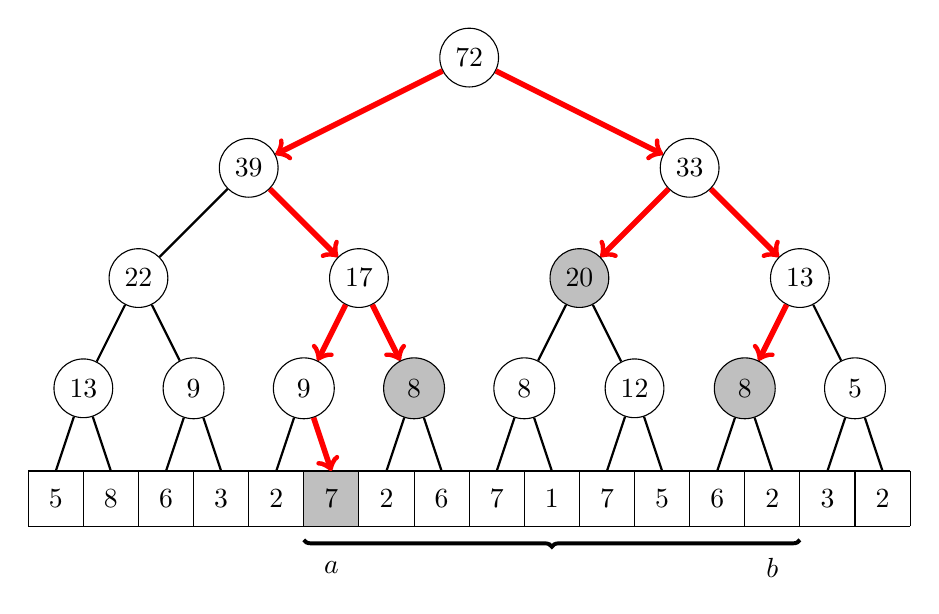
\begin{tikzpicture}[scale=0.7]
\fill[color=gray!50] (5,0) rectangle (6,1);
\draw (0,0) grid (16,1);

\node[anchor=center] at (0.5, 0.5) {5};
\node[anchor=center] at (1.5, 0.5) {8};
\node[anchor=center] at (2.5, 0.5) {6};
\node[anchor=center] at (3.5, 0.5) {3};
\node[anchor=center] at (4.5, 0.5) {2};
\node[anchor=center] at (5.5, 0.5) {7};
\node[anchor=center] at (6.5, 0.5) {2};
\node[anchor=center] at (7.5, 0.5) {6};
\node[anchor=center] at (8.5, 0.5) {7};
\node[anchor=center] at (9.5, 0.5) {1};
\node[anchor=center] at (10.5, 0.5) {7};
\node[anchor=center] at (11.5, 0.5) {5};
\node[anchor=center] at (12.5, 0.5) {6};
\node[anchor=center] at (13.5, 0.5) {2};
\node[anchor=center] at (14.5, 0.5) {3};
\node[anchor=center] at (15.5, 0.5) {2};

%\node[anchor=center] at (1,2.5) {13};

\node[draw, circle] (a) at (1,2.5) {13};
\path[draw,thick,-] (a) -- (0.5,1);
\path[draw,thick,-] (a) -- (1.5,1);
\node[draw, circle,minimum size=22pt] (b) at (3,2.5) {9};
\path[draw,thick,-] (b) -- (2.5,1);
\path[draw,thick,-] (b) -- (3.5,1);
\node[draw, circle,minimum size=22pt] (c) at (5,2.5) {9};
\path[draw,thick,-] (c) -- (4.5,1);
\path[draw,thick,-] (c) -- (5.5,1);
\node[draw, circle,fill=gray!50,minimum size=22pt] (d) at (7,2.5) {8};
\path[draw,thick,-] (d) -- (6.5,1);
\path[draw,thick,-] (d) -- (7.5,1);
\node[draw, circle,minimum size=22pt] (e) at (9,2.5) {8};
\path[draw,thick,-] (e) -- (8.5,1);
\path[draw,thick,-] (e) -- (9.5,1);
\node[draw, circle] (f) at (11,2.5) {12};
\path[draw,thick,-] (f) -- (10.5,1);
\path[draw,thick,-] (f) -- (11.5,1);
\node[draw, circle,fill=gray!50,minimum size=22pt] (g) at (13,2.5) {8};
\path[draw,thick,-] (g) -- (12.5,1);
\path[draw,thick,-] (g) -- (13.5,1);
\node[draw, circle,minimum size=22pt] (h) at (15,2.5) {5};
\path[draw,thick,-] (h) -- (14.5,1);
\path[draw,thick,-] (h) -- (15.5,1);

\node[draw, circle] (i) at (2,4.5) {22};
\path[draw,thick,-] (i) -- (a);
\path[draw,thick,-] (i) -- (b);
\node[draw, circle] (j) at (6,4.5) {17};
\path[draw,thick,-] (j) -- (c);
\path[draw,thick,-] (j) -- (d);
\node[draw, circle,fill=gray!50] (k) at (10,4.5) {20};
\path[draw,thick,-] (k) -- (e);
\path[draw,thick,-] (k) -- (f);
\node[draw, circle] (l) at (14,4.5) {13};
\path[draw,thick,-] (l) -- (g);
\path[draw,thick,-] (l) -- (h);

\node[draw, circle] (m) at (4,6.5) {39};
\path[draw,thick,-] (m) -- (i);
\path[draw,thick,-] (m) -- (j);
\node[draw, circle] (n) at (12,6.5) {33};
\path[draw,thick,-] (n) -- (k);
\path[draw,thick,-] (n) -- (l);

\node[draw, circle] (o) at (8,8.5) {72};
\path[draw,thick,-] (o) -- (m);
\path[draw,thick,-] (o) -- (n);

\path[draw=red,thick,->,line width=2pt] (o) -- (m);
\path[draw=red,thick,->,line width=2pt] (o) -- (n);

\path[draw=red,thick,->,line width=2pt] (m) -- (j);
\path[draw=red,thick,->,line width=2pt] (j) -- (c);
\path[draw=red,thick,->,line width=2pt] (j) -- (d);
\path[draw=red,thick,->,line width=2pt] (c) -- (5.5,1);

\path[draw=red,thick,->,line width=2pt] (n) -- (k);
\path[draw=red,thick,->,line width=2pt] (n) -- (l);

\path[draw=red,thick,->,line width=2pt] (l) -- (g);

\draw [decoration={brace}, decorate, line width=0.5mm] (14,-0.25) -- (5,-0.25);

\node at (5.5,-0.75) {$a$};
\node at (13.5,-0.75) {$b$};
\end{tikzpicture}
\end{center}

Também nesta implementação, as operações levam tempo $O(\log n)$, pois o número total de nós visitados é $O(\log n)$.

\section{Propagação preguiçosa}

\index{propagação preguiçosa}
\index{árvore de segmentos preguiçosa}

Usando \key{propagação preguiçosa}, podemos construir uma árvore de segmentos que suporta \emph{tanto} atualizações de intervalo quanto consultas de intervalo em tempo $O(\log n)$. A ideia é realizar atualizações e consultas de cima para baixo e realizar atualizações \emph{preguiçosamente}, de forma que sejam propagadas para baixo na árvore apenas quando necessário.

Em uma árvore de segmentos preguiçosa, os nós contêm dois tipos de informação. Como em uma árvore de segmentos comum, cada nó contém a soma ou algum outro valor relacionado ao subarray correspondente. Além disso, o nó pode conter informações relacionadas a atualizações preguiçosas, que não foram propagadas para seus filhos.

Existem dois tipos de atualizações de intervalo: cada valor do array no intervalo é \emph{aumentado} em algum valor ou \emph{atribuído} a algum valor. Ambas as operações podem ser implementadas usando ideias semelhantes e é até possível construir uma árvore que suporte ambas as operações ao mesmo tempo.

\subsubsection{Árvores de segmentos preguiçosas}

Vamos considerar um exemplo em que nosso objetivo é construir uma árvore de segmentos que suporte duas operações: aumentar cada valor em $[a,b]$ por uma constante e calcular a soma dos valores em $[a,b]$.

Vamos construir uma árvore onde cada nó tem dois valores $s/z$: $s$ denota a soma dos valores no intervalo e $z$ denota o valor de uma atualização preguiçosa, o que significa que todos os valores no intervalo devem ser aumentados em $z$. Na árvore a seguir, $z=0$ em todos os nós, portanto, não há atualizações preguiçosas em andamento.

\begin{center}
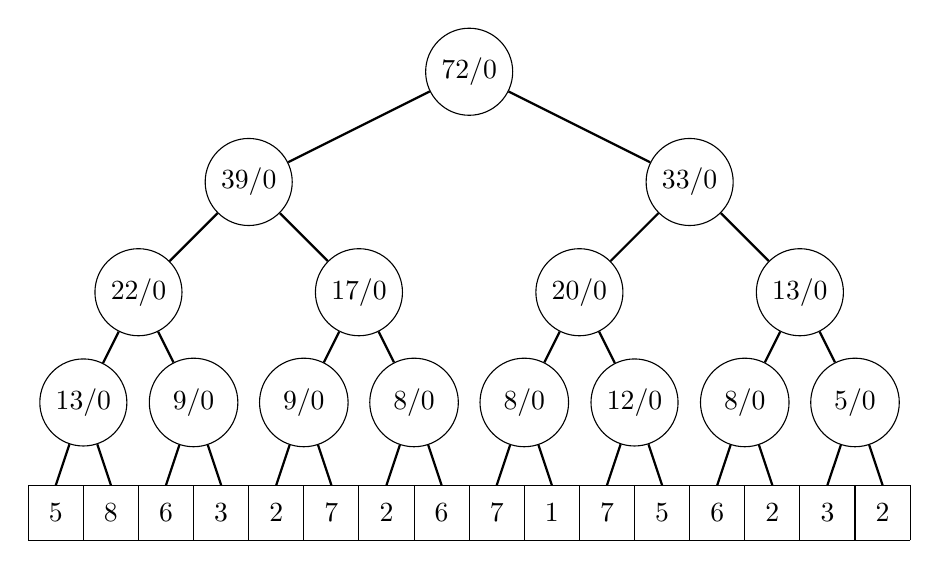
\begin{tikzpicture}[scale=0.7]
\draw (0,0) grid (16,1);

\node[anchor=center] at (0.5, 0.5) {5};
\node[anchor=center] at (1.5, 0.5) {8};
\node[anchor=center] at (2.5, 0.5) {6};
\node[anchor=center] at (3.5, 0.5) {3};
\node[anchor=center] at (4.5, 0.5) {2};
\node[anchor=center] at (5.5, 0.5) {7};
\node[anchor=center] at (6.5, 0.5) {2};
\node[anchor=center] at (7.5, 0.5) {6};
\node[anchor=center] at (8.5, 0.5) {7};
\node[anchor=center] at (9.5, 0.5) {1};
\node[anchor=center] at (10.5, 0.5) {7};
\node[anchor=center] at (11.5, 0.5) {5};
\node[anchor=center] at (12.5, 0.5) {6};
\node[anchor=center] at (13.5, 0.5) {2};
\node[anchor=center] at (14.5, 0.5) {3};
\node[anchor=center] at (15.5, 0.5) {2};

\node[draw, circle] (a) at (1,2.5) {13/0};
\path[draw,thick,-] (a) -- (0.5,1);
\path[draw,thick,-] (a) -- (1.5,1);
\node[draw, circle,minimum size=32pt] (b) at (3,2.5) {9/0};
\path[draw,thick,-] (b) -- (2.5,1);
\path[draw,thick,-] (b) -- (3.5,1);
\node[draw, circle,minimum size=32pt] (c) at (5,2.5) {9/0};
\path[draw,thick,-] (c) -- (4.5,1);
\path[draw,thick,-] (c) -- (5.5,1);
\node[draw, circle,minimum size=32pt] (d) at (7,2.5) {8/0};
\path[draw,thick,-] (d) -- (6.5,1);
\path[draw,thick,-] (d) -- (7.5,1);
\node[draw, circle,minimum size=32pt] (e) at (9,2.5) {8/0};
\path[draw,thick,-] (e) -- (8.5,1);
\path[draw,thick,-] (e) -- (9.5,1);
\node[draw, circle] (f) at (11,2.5) {12/0};
\path[draw,thick,-] (f) -- (10.5,1);
\path[draw,thick,-] (f) -- (11.5,1);
\node[draw, circle,minimum size=32pt] (g) at (13,2.5) {8/0};
\path[draw,thick,-] (g) -- (12.5,1);
\path[draw,thick,-] (g) -- (13.5,1);
\node[draw, circle,minimum size=32pt] (h) at (15,2.5) {5/0};
\path[draw,thick,-] (h) -- (14.5,1);
\path[draw,thick,-] (h) -- (15.5,1);

\node[draw, circle] (i) at (2,4.5) {22/0};
\path[draw,thick,-] (i) -- (a);
\path[draw,thick,-] (i) -- (b);
\node[draw, circle] (j) at (6,4.5) {17/0};
\path[draw,thick,-] (j) -- (c);
\path[draw,thick,-] (j) -- (d);
\node[draw, circle] (k) at (10,4.5) {20/0};
\path[draw,thick,-] (k) -- (e);
\path[draw,thick,-] (k) -- (f);
\node[draw, circle] (l) at (14,4.5) {13/0};
\path[draw,thick,-] (l) -- (g);
\path[draw,thick,-] (l) -- (h);

\node[draw, circle] (m) at (4,6.5) {39/0};
\path[draw,thick,-] (m) -- (i);
\path[draw,thick,-] (m) -- (j);
\node[draw, circle] (n) at (12,6.5) {33/0};
\path[draw,thick,-] (n) -- (k);
\path[draw,thick,-] (n) -- (l);

\node[draw, circle] (o) at (8,8.5) {72/0};
\path[draw,thick,-] (o) -- (m);
\path[draw,thick,-] (o) -- (n);
\end{tikzpicture}
\end{center}

Quando os elementos em $[a,b]$ são aumentados em $u$, caminhamos da raiz em direção às folhas e modificamos os nós da árvore da seguinte forma: Se o intervalo $[x,y]$ de um nó estiver completamente dentro de $[a,b]$, aumentamos o valor $z$ do nó em $u$ e paramos. Se $[x,y]$ pertencer apenas parcialmente a $[a,b]$, aumentamos o valor $s$ do nó em $hu$, onde $h$ é o tamanho da interseção de $[a,b]$ e $[x,y]$ e continuamos nossa caminhada recursivamente na árvore.

Por exemplo, a figura a seguir mostra a árvore após aumentar os elementos em $[a,b]$ em 2:

\begin{center}
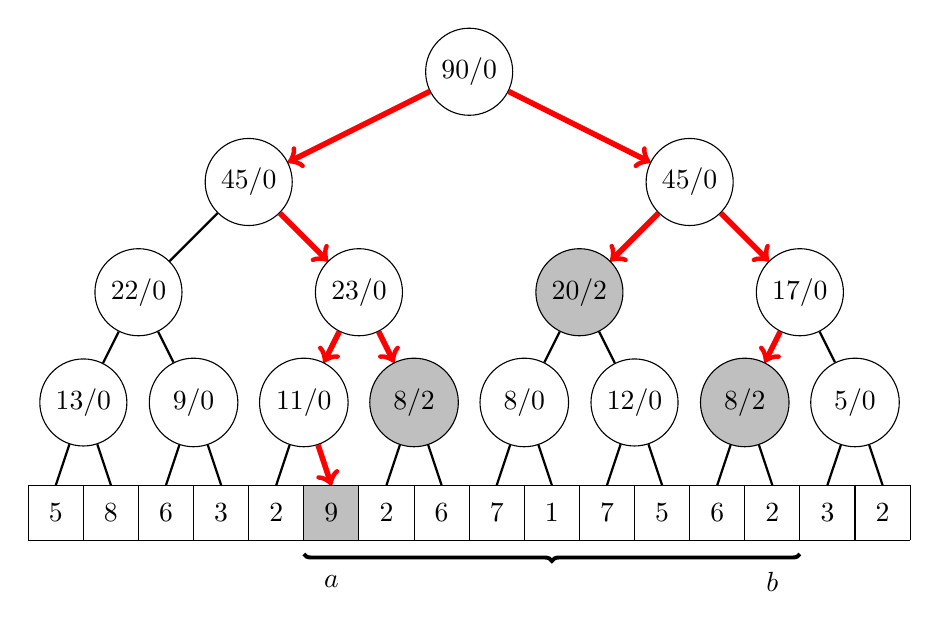
\begin{tikzpicture}[scale=0.7]
\fill[color=gray!50] (5,0) rectangle (6,1);
\draw (0,0) grid (16,1);

\node[anchor=center] at (0.5, 0.5) {5};
\node[anchor=center] at (1.5, 0.5) {8};
\node[anchor=center] at (2.5, 0.5) {6};
\node[anchor=center] at (3.5, 0.5) {3};
\node[anchor=center] at (4.5, 0.5) {2};
\node[anchor=center] at (5.5, 0.5) {9};
\node[anchor=center] at (6.5, 0.5) {2};
\node[anchor=center] at (7.5, 0.5) {6};
\node[anchor=center] at (8.5, 0.5) {7};
\node[anchor=center] at (9.5, 0.5) {1};
\node[anchor=center] at (10.5, 0.5) {7};
\node[anchor=center] at (11.5, 0.5) {5};
\node[anchor=center] at (12.5, 0.5) {6};
\node[anchor=center] at (13.5, 0.5) {2};
\node[anchor=center] at (14.5, 0.5) {3};
\node[anchor=center] at (15.5, 0.5) {2};

\node[draw, circle] (a) at (1,2.5) {13/0};
\path[draw,thick,-] (a) -- (0.5,1);
\path[draw,thick,-] (a) -- (1.5,1);
\node[draw, circle,minimum size=32pt] (b) at (3,2.5) {9/0};
\path[draw,thick,-] (b) -- (2.5,1);
\path[draw,thick,-] (b) -- (3.5,1);
\node[draw, circle,minimum size=32pt] (c) at (5,2.5) {11/0};
\path[draw,thick,-] (c) -- (4.5,1);
\path[draw,thick,-] (c) -- (5.5,1);
\node[draw, circle,fill=gray!50,minimum size=32pt] (d) at (7,2.5) {8/2};
\path[draw,thick,-] (d) -- (6.5,1);
\path[draw,thick,-] (d) -- (7.5,1);
\node[draw, circle,minimum size=32pt] (e) at (9,2.5) {8/0};
\path[draw,thick,-] (e) -- (8.5,1);
\path[draw,thick,-] (e) -- (9.5,1);
\node[draw, circle] (f) at (11,2.5) {12/0};
\path[draw,thick,-] (f) -- (10.5,1);
\path[draw,thick,-] (f) -- (11.5,1);
\node[draw, circle,fill=gray!50,minimum size=32pt] (g) at (13,2.5) {8/2};
\path[draw,thick,-] (g) -- (12.5,1);
\path[draw,thick,-] (g) -- (13.5,1);
\node[draw, circle,minimum size=32pt] (h) at (15,2.5) {5/0};
\path[draw,thick,-] (h) -- (14.5,1);
\path[draw,thick,-] (h) -- (15.5,1);

\node[draw, circle] (i) at (2,4.5) {22/0};
\path[draw,thick,-] (i) -- (a);
\path[draw,thick,-] (i) -- (b);
\node[draw, circle] (j) at (6,4.5) {23/0};
\path[draw,thick,-] (j) -- (c);
\path[draw,thick,-] (j) -- (d);
\node[draw, circle,fill=gray!50] (k) at (10,4.5) {20/2};
\path[draw,thick,-] (k) -- (e);
\path[draw,thick,-] (k) -- (f);
\node[draw, circle] (l) at (14,4.5) {17/0};
\path[draw,thick,-] (l) -- (g);
\path[draw,thick,-] (l) -- (h);

\node[draw, circle] (m) at (4,6.5) {45/0};
\path[draw,thick,-] (m) -- (i);
\path[draw,thick,-] (m) -- (j);
\node[draw, circle] (n) at (12,6.5) {45/0};
\path[draw,thick,-] (n) -- (k);
\path[draw,thick,-] (n) -- (l);

\node[draw, circle] (o) at (8,8.5) {90/0};
\path[draw,thick,-] (o) -- (m);
\path[draw,thick,-] (o) -- (n);

\path[draw=red,thick,->,line width=2pt] (o) -- (m);
\path[draw=red,thick,->,line width=2pt] (o) -- (n);

\path[draw=red,thick,->,line width=2pt] (m) -- (j);
\path[draw=red,thick,->,line width=2pt] (j) -- (c);
\path[draw=red,thick,->,line width=2pt] (j) -- (d);
\path[draw=red,thick,->,line width=2pt] (c) -- (5.5,1);

\path[draw=red,thick,->,line width=2pt] (n) -- (k);
\path[draw=red,thick,->,line width=2pt] (n) -- (l);

\path[draw=red,thick,->,line width=2pt] (l) -- (g);

\draw [decoration={brace}, decorate, line width=0.5mm] (14,-0.25) -- (5,-0.25);

\node at (5.5,-0.75) {$a$};
\node at (13.5,-0.75) {$b$};
\end{tikzpicture}
\end{center}

Também calculamos a soma dos elementos em um intervalo $[a,b]$ caminhando na árvore de cima para baixo. Se o intervalo $[x,y]$ de um nó pertencer completamente a $[a,b]$, adicionamos o valor $s$ do nó à soma. Caso contrário, continuamos a busca recursivamente para baixo na árvore.

Tanto nas atualizações quanto nas consultas, o valor de uma atualização preguiçosa é sempre propagado para os filhos do nó antes de processar o nó. A ideia é que as atualizações sejam propagadas para baixo apenas quando necessário, o que garante que as operações sejam sempre eficientes.

A figura a seguir mostra como a árvore muda quando calculamos o valor de $\texttt{sum}_a(a,b)$. O retângulo mostra os nós cujos valores mudam, porque uma atualização preguiçosa é propagada para baixo.

\begin{center}
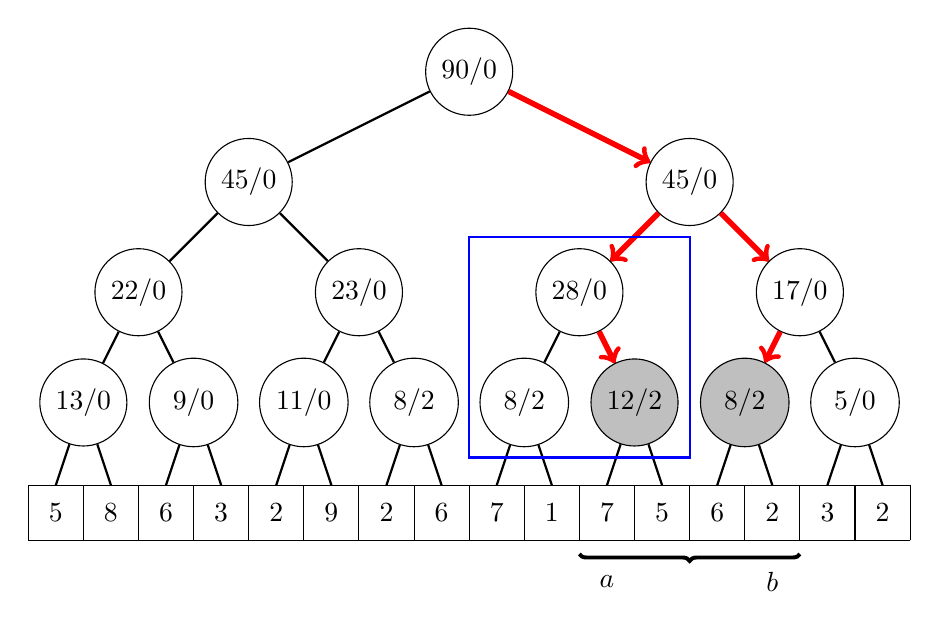
\begin{tikzpicture}[scale=0.7]
\draw (0,0) grid (16,1);

\node[anchor=center] at (0.5, 0.5) {5};
\node[anchor=center] at (1.5, 0.5) {8};
\node[anchor=center] at (2.5, 0.5) {6};
\node[anchor=center] at (3.5, 0.5) {3};
\node[anchor=center] at (4.5, 0.5) {2};
\node[anchor=center] at (5.5, 0.5) {9};
\node[anchor=center] at (6.5, 0.5) {2};
\node[anchor=center] at (7.5, 0.5) {6};
\node[anchor=center] at (8.5, 0.5) {7};
\node[anchor=center] at (9.5, 0.5) {1};
\node[anchor=center] at (10.5, 0.5) {7};
\node[anchor=center] at (11.5, 0.5) {5};
\node[anchor=center] at (12.5, 0.5) {6};
\node[anchor=center] at (13.5, 0.5) {2};
\node[anchor=center] at (14.5, 0.5) {3};
\node[anchor=center] at (15.5, 0.5) {2};

\node[draw, circle] (a) at (1,2.5) {13/0};
\path[draw,thick,-] (a) -- (0.5,1);
\path[draw,thick,-] (a) -- (1.5,1);
\node[draw, circle,minimum size=32pt] (b) at (3,2.5) {9/0};
\path[draw,thick,-] (b) -- (2.5,1);
\path[draw,thick,-] (b) -- (3.5,1);
\node[draw, circle,minimum size=32pt] (c) at (5,2.5) {11/0};
\path[draw,thick,-] (c) -- (4.5,1);
\path[draw,thick,-] (c) -- (5.5,1);
\node[draw, circle,minimum size=32pt] (d) at (7,2.5) {8/2};
\path[draw,thick,-] (d) -- (6.5,1);
\path[draw,thick,-] (d) -- (7.5,1);
\node[draw, circle,minimum size=32pt] (e) at (9,2.5) {8/2};
\path[draw,thick,-] (e) -- (8.5,1);
\path[draw,thick,-] (e) -- (9.5,1);
\node[draw, circle,fill=gray!50,] (f) at (11,2.5) {12/2};
\path[draw,thick,-] (f) -- (10.5,1);
\path[draw,thick,-] (f) -- (11.5,1);
\node[draw, circle,fill=gray!50,minimum size=32pt] (g) at (13,2.5) {8/2};
\path[draw,thick,-] (g) -- (12.5,1);
\path[draw,thick,-] (g) -- (13.5,1);
\node[draw, circle,minimum size=32pt] (h) at (15,2.5) {5/0};
\path[draw,thick,-] (h) -- (14.5,1);
\path[draw,thick,-] (h) -- (15.5,1);

\node[draw, circle] (i) at (2,4.5) {22/0};
\path[draw,thick,-] (i) -- (a);
\path[draw,thick,-] (i) -- (b);
\node[draw, circle] (j) at (6,4.5) {23/0};
\path[draw,thick,-] (j) -- (c);
\path[draw,thick,-] (j) -- (d);
\node[draw, circle] (k) at (10,4.5) {28/0};
\path[draw,thick,-] (k) -- (e);
\path[draw,thick,-] (k) -- (f);
\node[draw, circle] (l) at (14,4.5) {17/0};
\path[draw,thick,-] (l) -- (g);
\path[draw,thick,-] (l) -- (h);

\node[draw, circle] (m) at (4,6.5) {45/0};
\path[draw,thick,-] (m) -- (i);
\path[draw,thick,-] (m) -- (j);
\node[draw, circle] (n) at (12,6.5) {45/0};
\path[draw,thick,-] (n) -- (k);
\path[draw,thick,-] (n) -- (l);

\node[draw, circle] (o) at (8,8.5) {90/0};
\path[draw,thick,-] (o) -- (m);
\path[draw,thick,-] (o) -- (n);

\path[draw=red,thick,->,line width=2pt] (o) -- (n);

\path[draw=red,thick,->,line width=2pt] (n) -- (k);
\path[draw=red,thick,->,line width=2pt] (n) -- (l);

\path[draw=red,thick,->,line width=2pt] (k) -- (f);
\path[draw=red,thick,->,line width=2pt] (l) -- (g);

\draw [decoration={brace}, decorate, line width=0.5mm] (14,-0.25) -- (10,-0.25);

\draw[color=blue,thick] (8,1.5) rectangle (12,5.5);

\node at (10.5,-0.75) {$a$};
\node at (13.5,-0.75) {$b$};
\end{tikzpicture}
\end{center}

Observe que às vezes é necessário combinar atualizações preguiçosas. Isso acontece quando um nó que já possui uma atualização preguiçosa recebe outra atualização preguiçosa. Ao calcular as somas, é fácil combinar atualizações preguiçosas, pois a combinação das atualizações $z_1$ e $z_2$ corresponde a uma atualização $z_1+z_2$.

\subsubsection{Atualizações polinomiais}

As atualizações preguiçosas podem ser generalizadas para que seja possível atualizar intervalos usando polinômios da forma
\[p(u) = t_k u^k + t_{k-1} u^{k-1} + \cdots + t_0.\]

Nesse caso, a atualização de um valor na posição $i$ em $[a,b]$ é $p(i-a)$. Por exemplo, adicionar o polinômio $p(u)=u+1$ a $[a,b]$ significa que o valor na posição $a$ aumenta em 1, o valor na posição $a+1$ aumenta em 2 e assim por diante.

Para suportar atualizações polinomiais, cada nó recebe $k+2$ valores, onde $k$ é igual ao grau do polinômio. O valor $s$ é a soma dos elementos no intervalo e os valores $z_0,z_1,\ldots,z_k$ são os coeficientes de um polinômio que corresponde a uma atualização preguiçosa

Agora, a soma dos valores em um intervalo $[x,y]$ é igual a
\[s+\sum_{u=0}^{y-x} z_k u^k + z_{k-1} u^{k-1} + \cdots + z_0.\]

O valor de tal soma pode ser calculado eficientemente usando fórmulas de soma. Por exemplo, o termo $z_0$ corresponde à soma $(y-x+1)z_0$ e o termo $z_1 u$ corresponde à soma
\[z_1(0+1+\cdots+y-x) = z_1 \frac{(y-x)(y-x+1)}{2} .\]

Ao propagar uma atualização na árvore, os índices de $p(u)$ mudam, pois em cada intervalo $[x,y]$, os valores são calculados para $u=0,1,\ldots,y-x$. No entanto, isso não é um problema, pois $p'(u)=p(u+h)$ é um polinômio de mesmo grau que $p(u)$. Por exemplo, se $p(u)=t_2 u^2+t_1 u-t_0$, então
\[p'(u)=t_2(u+h)^2+t_1(u+h)-t_0=t_2 u^2 + (2ht_2+t_1)u+t_2h^2+t_1h-t_0.\]

\section{Árvores dinâmicas}

\index{árvore de segmentos dinâmica}

Uma árvore de segmentos comum é estática, o que significa que cada nó tem uma posição fixa no array e a árvore requer uma quantidade fixa de memória. Em uma \key{árvore de segmentos dinâmica}, a memória é alocada apenas para nós que são realmente acessados durante o algoritmo, o que pode economizar uma grande quantidade de memória.

Os nós de uma árvore dinâmica podem ser representados como structs:
\begin{lstlisting}
struct node {
    int value;
    int x, y;
    node *left, *right;
    node(int v, int x, int y) : value(v), x(x), y(y) {}
};
\end{lstlisting}
Aqui, \texttt{value} é o valor do nó, $[\texttt{x},\texttt{y}]$ é o intervalo correspondente e \texttt{left} e \texttt{right} apontam para a subárvore esquerda e direita.

Depois disso, os nós podem ser criados da seguinte forma:
\begin{lstlisting}
// cria um novo no
node *x = new node(0, 0, 15);
// altera o valor
x->value = 5;
\end{lstlisting}

\subsubsection{Árvores de segmentos esparsas}

\index{árvore de segmentos esparsa}

Uma árvore de segmentos dinâmica é útil quando o array subjacente é \emph{esparso}, ou seja, o intervalo $[0,n-1]$ de índices permitidos é grande, mas a maioria dos valores do array são zeros. Enquanto uma árvore de segmentos comum usa memória $O(n)$, uma árvore de segmentos dinâmica usa apenas memória $O(k \log n)$, onde $k$ é o número de operações realizadas.

Uma \key{árvore de segmentos esparsa} inicialmente tem apenas um nó $[0,n-1]$ cujo valor é zero, o que significa que todos os valores do array são zero. Após as atualizações, novos nós são adicionados dinamicamente à árvore. Por exemplo, se $n=16$ e os elementos nas posições 3 e 10 foram modificados, a árvore contém os seguintes nós:
\begin{center}
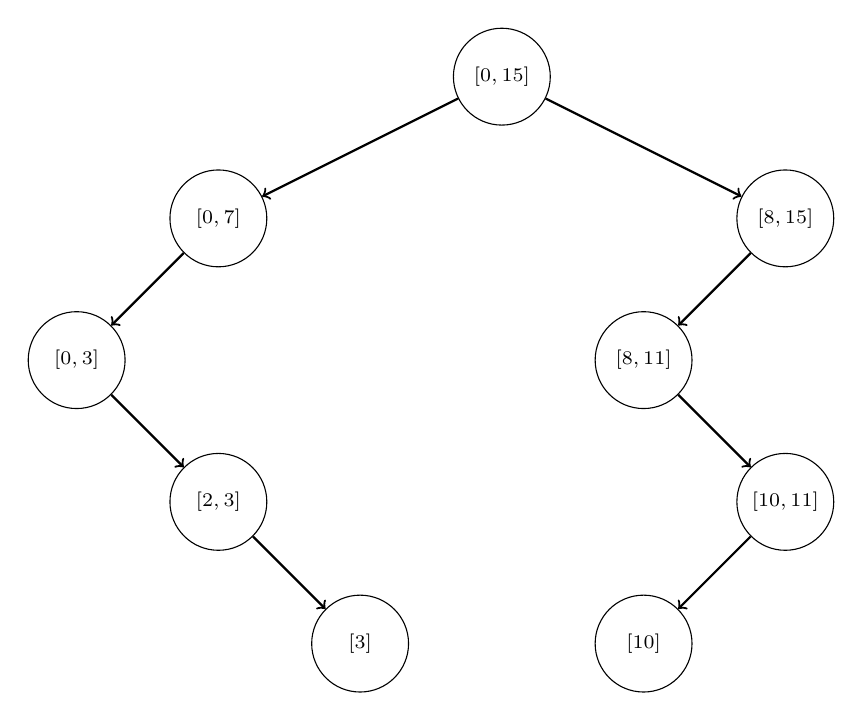
\begin{tikzpicture}[scale=0.9]
\scriptsize
\node[draw, circle,minimum size=35pt] (1) at (0,0) {$[0,15]$};
\node[draw, circle,minimum size=35pt] (2) at (-4,-2) {$[0,7]$};
\node[draw, circle,minimum size=35pt] (3) at (-6,-4) {$[0,3]$};
\node[draw, circle,minimum size=35pt] (4) at (-4,-6) {$[2,3]$};
\node[draw, circle,minimum size=35pt] (5) at (-2,-8) {$[3]$};
\node[draw, circle,minimum size=35pt] (6) at (4,-2) {$[8,15]$};
\node[draw, circle,minimum size=35pt] (7) at (2,-4) {$[8,11]$};
\node[draw, circle,minimum size=35pt] (8) at (4,-6) {$[10,11]$};
\node[draw, circle,minimum size=35pt] (9) at (2,-8) {$[10]$};

\path[draw,thick,->] (1) -- (2);
\path[draw,thick,->] (2) -- (3);
\path[draw,thick,->] (3) -- (4);
\path[draw,thick,->] (4) -- (5);

\path[draw,thick,->] (1) -- (6);
\path[draw,thick,->] (6) -- (7);
\path[draw,thick,->] (7) -- (8);
\path[draw,thick,->] (8) -- (9);
\end{tikzpicture}
\end{center}

Qualquer caminho do nó raiz a uma folha contém $O(\log n)$ nós, então cada operação adiciona no máximo $O(\log n)$ novos nós à árvore. Assim, após $k$ operações, a árvore contém no máximo $O(k \log n)$ nós.

Observe que, se soubermos todos os elementos a serem atualizados no início do algoritmo, uma árvore de segmentos dinâmica não será necessária, pois podemos usar uma árvore de segmentos comum com compressão de índice (Capítulo 9.4). No entanto, isso não é possível quando os índices são gerados durante o algoritmo.

\subsubsection{Árvores de segmentos persistentes}

\index{árvore de segmentos persistente}

Usando uma implementação dinâmica, também é possível criar uma \key{árvore de segmentos persistente} que armazena o \emph{histórico de modificações} da árvore. Em tal implementação, podemos acessar com eficiência todas as versões da árvore que existiram durante o algoritmo.

Quando o histórico de modificações está disponível, podemos realizar consultas em qualquer árvore anterior como em uma árvore de segmentos comum, pois a estrutura completa de cada árvore é armazenada. Também podemos criar novas árvores com base em árvores anteriores e modificá-las independentemente.

Considere a seguinte sequência de atualizações, onde os nós vermelhos mudam e os outros nós permanecem os mesmos:

\begin{center}
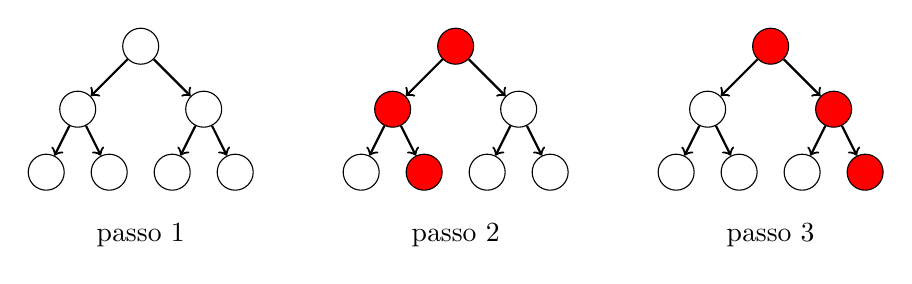
\begin{tikzpicture}[scale=0.8]
\node[draw, circle,minimum size=13pt] (1a) at (3,0) {};
\node[draw, circle,minimum size=13pt] (2a) at (2,-1) {};
\node[draw, circle,minimum size=13pt] (3a) at (4,-1) {};
\node[draw, circle,minimum size=13pt] (4a) at (1.5,-2) {};
\node[draw, circle,minimum size=13pt] (5a) at (2.5,-2) {};
\node[draw, circle,minimum size=13pt] (6a) at (3.5,-2) {};
\node[draw, circle,minimum size=13pt] (7a) at (4.5,-2) {};
\path[draw,thick,->] (1a) -- (2a);
\path[draw,thick,->] (1a) -- (3a);
\path[draw,thick,->] (2a) -- (4a);
\path[draw,thick,->] (2a) -- (5a);
\path[draw,thick,->] (3a) -- (6a);
\path[draw,thick,->] (3a) -- (7a);

\node[draw, circle,minimum size=13pt,fill=red] (1b) at (3+5,0) {};
\node[draw, circle,minimum size=13pt,fill=red] (2b) at (2+5,-1) {};
\node[draw, circle,minimum size=13pt] (3b) at (4+5,-1) {};
\node[draw, circle,minimum size=13pt] (4b) at (1.5+5,-2) {};
\node[draw, circle,minimum size=13pt,fill=red] (5b) at (2.5+5,-2) {};
\node[draw, circle,minimum size=13pt] (6b) at (3.5+5,-2) {};
\node[draw, circle,minimum size=13pt] (7b) at (4.5+5,-2) {};
\path[draw,thick,->] (1b) -- (2b);
\path[draw,thick,->] (1b) -- (3b);
\path[draw,thick,->] (2b) -- (4b);
\path[draw,thick,->] (2b) -- (5b);
\path[draw,thick,->] (3b) -- (6b);
\path[draw,thick,->] (3b) -- (7b);

\node[draw, circle,minimum size=13pt,fill=red] (1c) at (3+10,0) {};
\node[draw, circle,minimum size=13pt] (2c) at (2+10,-1) {};
\node[draw, circle,minimum size=13pt,fill=red] (3c) at (4+10,-1) {};
\node[draw, circle,minimum size=13pt] (4c) at (1.5+10,-2) {};
\node[draw, circle,minimum size=13pt] (5c) at (2.5+10,-2) {};
\node[draw, circle,minimum size=13pt] (6c) at (3.5+10,-2) {};
\node[draw, circle,minimum size=13pt,fill=red] (7c) at (4.5+10,-2) {};
\path[draw,thick,->] (1c) -- (2c);
\path[draw,thick,->] (1c) -- (3c);
\path[draw,thick,->] (2c) -- (4c);
\path[draw,thick,->] (2c) -- (5c);
\path[draw,thick,->] (3c) -- (6c);
\path[draw,thick,->] (3c) -- (7c);

\node at (3,-3) {passo 1};
\node at (3+5,-3) {passo 2};
\node at (3+10,-3) {passo 3};
\end{tikzpicture}
\end{center}

Após cada atualização, a maioria dos nós da árvore permanece a mesma, então uma maneira eficiente de armazenar o histórico de modificações é representar cada árvore no histórico como uma combinação de novos nós e subárvores de árvores anteriores. Neste exemplo, o histórico de modificações pode ser armazenado da seguinte forma:

\begin{center}
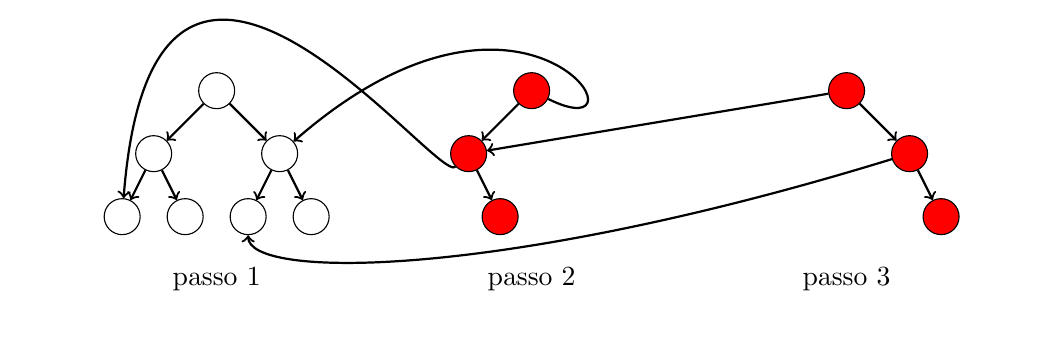
\begin{tikzpicture}[scale=0.8]
\path[use as bounding box] (0, 1) rectangle (16, -3.5);

\node[draw, circle,minimum size=13pt] (1a) at (3,0) {};
\node[draw, circle,minimum size=13pt] (2a) at (2,-1) {};
\node[draw, circle,minimum size=13pt] (3a) at (4,-1) {};
\node[draw, circle,minimum size=13pt] (4a) at (1.5,-2) {};
\node[draw, circle,minimum size=13pt] (5a) at (2.5,-2) {};
\node[draw, circle,minimum size=13pt] (6a) at (3.5,-2) {};
\node[draw, circle,minimum size=13pt] (7a) at (4.5,-2) {};
\path[draw,thick,->] (1a) -- (2a);
\path[draw,thick,->] (1a) -- (3a);
\path[draw,thick,->] (2a) -- (4a);
\path[draw,thick,->] (2a) -- (5a);
\path[draw,thick,->] (3a) -- (6a);
\path[draw,thick,->] (3a) -- (7a);

\node[draw, circle,minimum size=13pt,fill=red] (1b) at (3+5,0) {};
\node[draw, circle,minimum size=13pt,fill=red] (2b) at (2+5,-1) {};
\node[draw, circle,minimum size=13pt,fill=red] (5b) at (2.5+5,-2) {};
\path[draw,thick,->] (1b) -- (2b);

\draw[thick,->] (1b) .. controls (3+5+2,0-1) and (3+5,2.5) .. (3a);

\draw[thick,->] (2b) .. controls (2+5-0.5,-1-0.5) and (2,4.5) .. (4a);


\path[draw,thick,->] (2b) -- (5b);

\node[draw, circle,minimum size=13pt,fill=red] (1c) at (3+10,0) {};
\node[draw, circle,minimum size=13pt,fill=red] (3c) at (4+10,-1) {};
\node[draw, circle,minimum size=13pt,fill=red] (7c) at (4.5+10,-2) {};
\path[draw,thick,->] (1c) -- (2b);
\path[draw,thick,->] (1c) -- (3c);

\draw[thick,->] (3c) .. controls (2.5+5,-3) and (3.5,-3) .. (6a);

\path[draw,thick,->] (3c) -- (7c);

\node at (3,-3) {passo 1};
\node at (3+5,-3) {passo 2};
\node at (3+10,-3) {passo 3};
\end{tikzpicture}
\end{center}

A estrutura de cada árvore anterior pode ser reconstruída seguindo os ponteiros a partir do nó raiz correspondente. Como cada operação adiciona apenas $O(\log n)$ novos nós à árvore, é possível armazenar todo o histórico de modificações da árvore.

\section{Estruturas de dados}

Em vez de valores únicos, os nós em uma árvore de segmentos também podem conter \emph{estruturas de dados} que mantêm informações sobre os intervalos correspondentes. Em tal árvore, as operações levam tempo $O(f(n) \log n)$, onde $f(n)$ é o tempo necessário para processar um único nó durante uma operação.

Como exemplo, considere uma árvore de segmentos que suporta consultas da forma "quantas vezes um elemento $x$ aparece no intervalo $[a,b]$?" Por exemplo, o elemento 1 aparece três vezes no intervalo a seguir:

\begin{center}
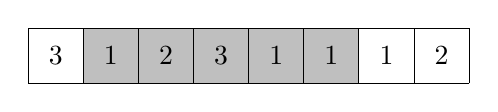
\begin{tikzpicture}[scale=0.7]
\fill[lightgray] (1,0) rectangle (6,1);
\draw (0,0) grid (8,1);

\node[anchor=center] at (0.5, 0.5) {3};
\node[anchor=center] at (1.5, 0.5) {1};
\node[anchor=center] at (2.5, 0.5) {2};
\node[anchor=center] at (3.5, 0.5) {3};
\node[anchor=center] at (4.5, 0.5) {1};
\node[anchor=center] at (5.5, 0.5) {1};
\node[anchor=center] at (6.5, 0.5) {1};
\node[anchor=center] at (7.5, 0.5) {2};
\end{tikzpicture}
\end{center}

Para suportar tais consultas, construímos uma árvore de segmentos onde cada nó é associado a uma estrutura de dados que pode ser consultada sobre quantas vezes qualquer elemento $x$ aparece no intervalo correspondente. Usando essa árvore, a resposta a uma consulta pode ser calculada combinando os resultados dos nós que pertencem ao intervalo.

Por exemplo, a seguinte árvore de segmentos corresponde ao array acima:
\begin{center}
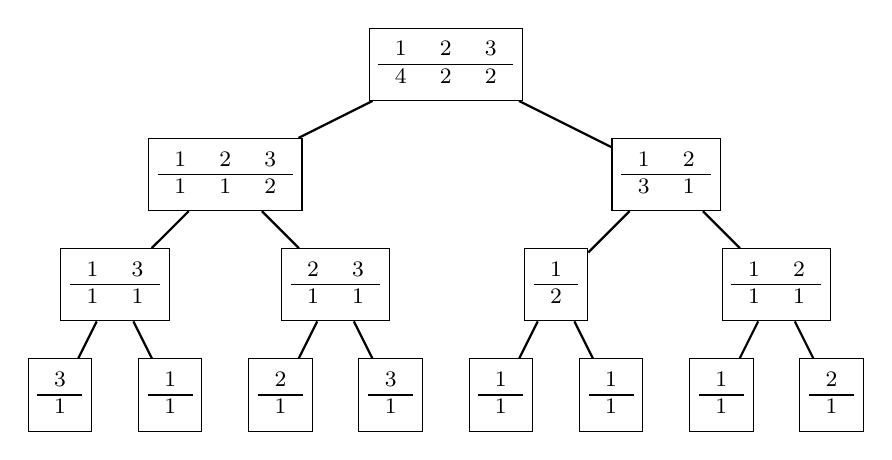
\begin{tikzpicture}[scale=0.7]

\node[draw, rectangle] (a) at (1,2.5)
{
\footnotesize
\begin{tabular}{r}
3 \\
\hline
1 \\
\end{tabular}};
\node[draw, rectangle] (b) at (3,2.5)
{
\footnotesize
\begin{tabular}{r}
1 \\
\hline
1 \\
\end{tabular}};
\node[draw, rectangle] (c) at (5,2.5)
{
\footnotesize
\begin{tabular}{r}
2 \\
\hline
1 \\
\end{tabular}};
\node[draw, rectangle] (d) at (7,2.5)
{
\footnotesize
\begin{tabular}{r}
3 \\
\hline
1 \\
\end{tabular}};
\node[draw, rectangle] (e) at (9,2.5)
{
\footnotesize
\begin{tabular}{r}
1 \\
\hline
1 \\
\end{tabular}};
\node[draw, rectangle] (f) at (11,2.5)
{
\footnotesize
\begin{tabular}{r}
1 \\
\hline
1 \\
\end{tabular}};
\node[draw, rectangle] (g) at (13,2.5)
{
\footnotesize
\begin{tabular}{r}
1 \\
\hline
1 \\
\end{tabular}};
\node[draw, rectangle] (h) at (15,2.5)
{
\footnotesize
\begin{tabular}{r}
2 \\
\hline
1 \\
\end{tabular}};

\node[draw, rectangle] (i) at (2,4.5)
{
\footnotesize
\begin{tabular}{rr}
1 & 3 \\
\hline
1 & 1 \\
\end{tabular}};
\path[draw,thick,-] (i) -- (a);
\path[draw,thick,-] (i) -- (b);
\node[draw, rectangle] (j) at (6,4.5)
{
\footnotesize
\begin{tabular}{rr}
2 & 3 \\
\hline
1 & 1 \\
\end{tabular}};
\path[draw,thick,-] (j) -- (c);
\path[draw,thick,-] (j) -- (d);
\node[draw, rectangle] (k) at (10,4.5)
{
\footnotesize
\begin{tabular}{r}
1 \\
\hline
2 \\
\end{tabular}};
\path[draw,thick,-] (k) -- (e);
\path[draw,thick,-] (k) -- (f);
\node[draw, rectangle] (l) at (14,4.5)
{
\footnotesize
\begin{tabular}{rr}
1 & 2 \\
\hline
1 & 1 \\
\end{tabular}};
\path[draw,thick,-] (l) -- (g);
\path[draw,thick,-] (l) -- (h);

\node[draw, rectangle] (m) at (4,6.5)
{
\footnotesize
\begin{tabular}{rrr}
1 & 2 & 3 \\
\hline
1 & 1 & 2 \\
\end{tabular}};
\path[draw,thick,-] (m) -- (i);
\path[draw,thick,-] (m) -- (j);
\node[draw, rectangle] (n) at (12,6.5)
{
\footnotesize
\begin{tabular}{rr}
1 & 2 \\
\hline
3 & 1 \\
\end{tabular}};
\path[draw,thick,-] (n) -- (k);
\path[draw,thick,-] (n) -- (l);

\node[draw, rectangle] (o) at (8,8.5)
{
\footnotesize
\begin{tabular}{rrr}
1 & 2 & 3 \\
\hline
4 & 2 & 2 \\
\end{tabular}};
\path[draw,thick,-] (o) -- (m);
\path[draw,thick,-] (o) -- (n);
\end{tikzpicture}
\end{center}

Podemos construir a árvore de forma que cada nó contenha uma estrutura de \texttt{map}. Nesse caso, o tempo necessário para processar cada nó é $O(\log n)$, então a complexidade de tempo total de uma consulta é $O(\log^2 n)$. A árvore usa memória $O(n \log n)$, pois existem $O(\log n)$ níveis e cada nível contém $O(n)$ elementos.

\section{Bidimensionalidade}

\index{árvore de segmentos bidimensional}

Uma \key{árvore de segmentos bidimensional} suporta consultas relacionadas a submatrizes retangulares de um array bidimensional. Essa árvore pode ser implementada como árvores de segmentos aninhadas: uma árvore grande corresponde às linhas do array e cada nó contém uma árvore pequena que corresponde a uma coluna.

Por exemplo, no array
\begin{center}
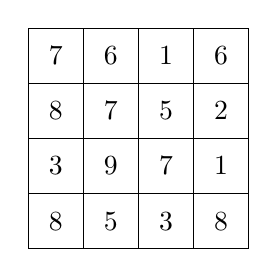
\begin{tikzpicture}[scale=0.7]
\draw (0,0) grid (4,4);

\node[anchor=center] at (0.5, 0.5) {8};
\node[anchor=center] at (1.5, 0.5) {5};
\node[anchor=center] at (2.5, 0.5) {3};
\node[anchor=center] at (3.5, 0.5) {8};

\node[anchor=center] at (0.5, 1.5) {3};
\node[anchor=center] at (1.5, 1.5) {9};
\node[anchor=center] at (2.5, 1.5) {7};
\node[anchor=center] at (3.5, 1.5) {1};

\node[anchor=center] at (0.5, 2.5) {8};
\node[anchor=center] at (1.5, 2.5) {7};
\node[anchor=center] at (2.5, 2.5) {5};
\node[anchor=center] at (3.5, 2.5) {2};

\node[anchor=center] at (0.5, 3.5) {7};
\node[anchor=center] at (1.5, 3.5) {6};
\node[anchor=center] at (2.5, 3.5) {1};
\node[anchor=center] at (3.5, 3.5) {6};
\end{tikzpicture}
\end{center}

a soma de qualquer submatriz pode ser calculada a partir da seguinte árvore de segmentos:

\begin{center}
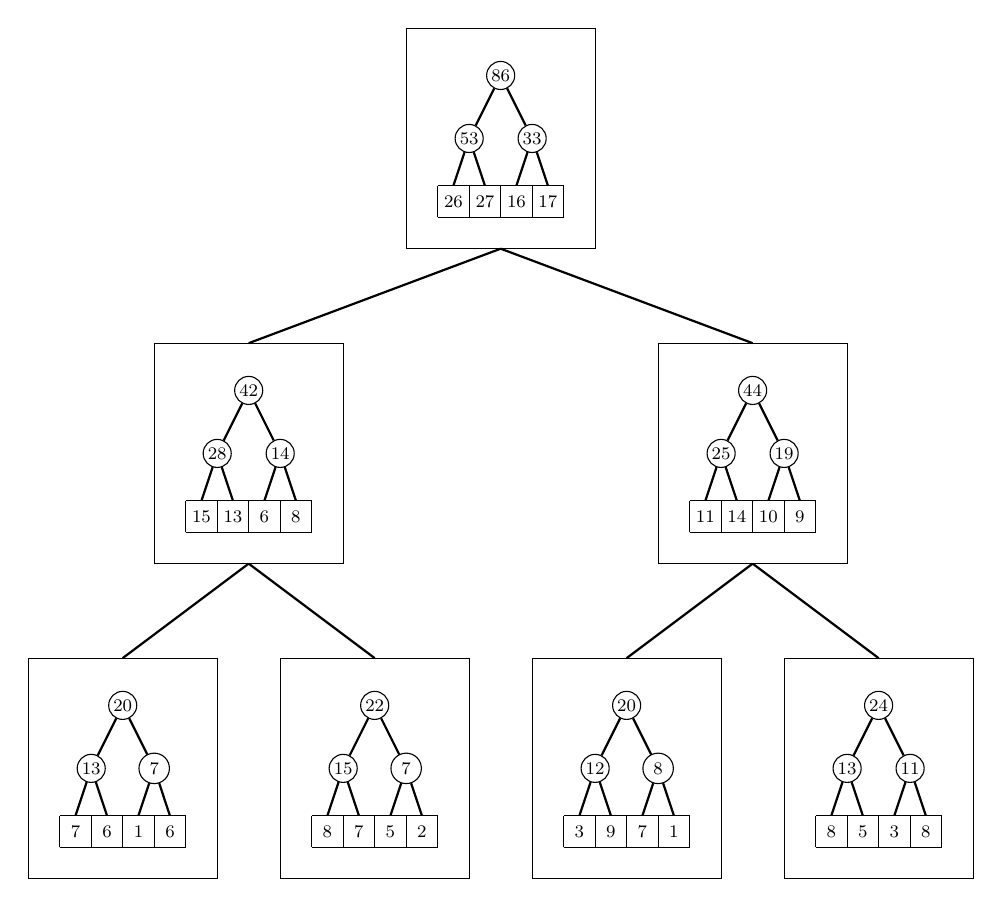
\begin{tikzpicture}[scale=0.4]
\footnotesize
\begin{scope}[shift={(-12,0)}]
\draw (-1,-1) rectangle (5,6);
\draw (0,0) grid (4,1);
\node[anchor=center,scale=0.8] at (0.5, 0.5) {7};
\node[anchor=center,scale=0.8] at (1.5, 0.5) {6};
\node[anchor=center,scale=0.8] at (2.5, 0.5) {1};
\node[anchor=center,scale=0.8] at (3.5, 0.5) {6};

\node[draw, circle,scale=0.8,inner sep=1pt] (a) at (1,2.5) {13};
\path[draw,thick,-] (a) -- (0.5,1);
\path[draw,thick,-] (a) -- (1.5,1);
\node[draw, circle,scale=0.8,inner sep=2.5pt] (b) at (3,2.5) {7};
\path[draw,thick,-] (b) -- (2.5,1);
\path[draw,thick,-] (b) -- (3.5,1);

\node[draw, circle,scale=0.8,inner sep=1pt] (i) at (2,4.5) {20};
\path[draw,thick,-] (i) -- (a);
\path[draw,thick,-] (i) -- (b);
\end{scope}
\begin{scope}[shift={(-4,0)}]
\draw (-1,-1) rectangle (5,6);
\draw (0,0) grid (4,1);
\node[anchor=center,scale=0.8] at (0.5, 0.5) {8};
\node[anchor=center,scale=0.8] at (1.5, 0.5) {7};
\node[anchor=center,scale=0.8] at (2.5, 0.5) {5};
\node[anchor=center,scale=0.8] at (3.5, 0.5) {2};

\node[draw, circle,scale=0.8,inner sep=1pt] (a) at (1,2.5) {15};
\path[draw,thick,-] (a) -- (0.5,1);
\path[draw,thick,-] (a) -- (1.5,1);
\node[draw, circle,scale=0.8,inner sep=2.5pt] (b) at (3,2.5) {7};
\path[draw,thick,-] (b) -- (2.5,1);
\path[draw,thick,-] (b) -- (3.5,1);

\node[draw, circle,scale=0.8,inner sep=1pt] (i) at (2,4.5) {22};
\path[draw,thick,-] (i) -- (a);
\path[draw,thick,-] (i) -- (b);
\end{scope}
\begin{scope}[shift={(4,0)}]
\draw (-1,-1) rectangle (5,6);
\draw (0,0) grid (4,1);
\node[anchor=center,scale=0.8] at (0.5, 0.5) {3};
\node[anchor=center,scale=0.8] at (1.5, 0.5) {9};
\node[anchor=center,scale=0.8] at (2.5, 0.5) {7};
\node[anchor=center,scale=0.8] at (3.5, 0.5) {1};

\node[draw, circle,scale=0.8,inner sep=1pt] (a) at (1,2.5) {12};
\path[draw,thick,-] (a) -- (0.5,1);
\path[draw,thick,-] (a) -- (1.5,1);
\node[draw, circle,scale=0.8,inner sep=2.5pt] (b) at (3,2.5) {8};
\path[draw,thick,-] (b) -- (2.5,1);
\path[draw,thick,-] (b) -- (3.5,1);

\node[draw, circle,scale=0.8,inner sep=1pt] (i) at (2,4.5) {20};
\path[draw,thick,-] (i) -- (a);
\path[draw,thick,-] (i) -- (b);
\end{scope}
\begin{scope}[shift={(12,0)}]
\draw (-1,-1) rectangle (5,6);
\draw (0,0) grid (4,1);
\node[anchor=center,scale=0.8] at (0.5, 0.5) {8};
\node[anchor=center,scale=0.8] at (1.5, 0.5) {5};
\node[anchor=center,scale=0.8] at (2.5, 0.5) {3};
\node[anchor=center,scale=0.8] at (3.5, 0.5) {8};

\node[draw, circle,scale=0.8,inner sep=1pt] (a) at (1,2.5) {13};
\path[draw,thick,-] (a) -- (0.5,1);
\path[draw,thick,-] (a) -- (1.5,1);
\node[draw, circle,scale=0.8,inner sep=1pt] (b) at (3,2.5) {11};
\path[draw,thick,-] (b) -- (2.5,1);
\path[draw,thick,-] (b) -- (3.5,1);

\node[draw, circle,scale=0.8,inner sep=1pt] (i) at (2,4.5) {24};
\path[draw,thick,-] (i) -- (a);
\path[draw,thick,-] (i) -- (b);
\end{scope}
\begin{scope}[shift={(-8,10)}]
\draw (-1,-1) rectangle (5,6);
\draw (0,0) grid (4,1);
\node[anchor=center,scale=0.8] at (0.5, 0.5) {15};
\node[anchor=center,scale=0.8] at (1.5, 0.5) {13};
\node[anchor=center,scale=0.8] at (2.5, 0.5) {6};
\node[anchor=center,scale=0.8] at (3.5, 0.5) {8};

\node[draw, circle,scale=0.8,inner sep=1pt] (a) at (1,2.5) {28};
\path[draw,thick,-] (a) -- (0.5,1);
\path[draw,thick,-] (a) -- (1.5,1);
\node[draw, circle,scale=0.8,inner sep=1pt] (b) at (3,2.5) {14};
\path[draw,thick,-] (b) -- (2.5,1);
\path[draw,thick,-] (b) -- (3.5,1);

\node[draw, circle,scale=0.8,inner sep=1pt] (i) at (2,4.5) {42};
\path[draw,thick,-] (i) -- (a);
\path[draw,thick,-] (i) -- (b);
\end{scope}
\begin{scope}[shift={(8,10)}]
\draw (-1,-1) rectangle (5,6);
\draw (0,0) grid (4,1);
\node[anchor=center,scale=0.8] at (0.5, 0.5) {11};
\node[anchor=center,scale=0.8] at (1.5, 0.5) {14};
\node[anchor=center,scale=0.8] at (2.5, 0.5) {10};
\node[anchor=center,scale=0.8] at (3.5, 0.5) {9};

\node[draw, circle,scale=0.8,inner sep=1pt] (a) at (1,2.5) {25};
\path[draw,thick,-] (a) -- (0.5,1);
\path[draw,thick,-] (a) -- (1.5,1);
\node[draw, circle,scale=0.8,inner sep=1pt] (b) at (3,2.5) {19};
\path[draw,thick,-] (b) -- (2.5,1);
\path[draw,thick,-] (b) -- (3.5,1);

\node[draw, circle,scale=0.8,inner sep=1pt] (i) at (2,4.5) {44};
\path[draw,thick,-] (i) -- (a);
\path[draw,thick,-] (i) -- (b);
\end{scope}
\begin{scope}[shift={(0,20)}]
\draw (-1,-1) rectangle (5,6);
\draw (0,0) grid (4,1);
\node[anchor=center,scale=0.8] at (0.5, 0.5) {26};
\node[anchor=center,scale=0.8] at (1.5, 0.5) {27};
\node[anchor=center,scale=0.8] at (2.5, 0.5) {16};
\node[anchor=center,scale=0.8] at (3.5, 0.5) {17};

\node[draw, circle,scale=0.8,inner sep=1pt] (a) at (1,2.5) {53};
\path[draw,thick,-] (a) -- (0.5,1);
\path[draw,thick,-] (a) -- (1.5,1);
\node[draw, circle,scale=0.8,inner sep=1pt] (b) at (3,2.5) {33};
\path[draw,thick,-] (b) -- (2.5,1);
\path[draw,thick,-] (b) -- (3.5,1);

\node[draw, circle,scale=0.8,inner sep=1pt] (i) at (2,4.5) {86};
\path[draw,thick,-] (i) -- (a);
\path[draw,thick,-] (i) -- (b);
\end{scope}
\path[draw,thick,-] (2,19) -- (-6,16);
\path[draw,thick,-] (2,19) -- (10,16);
\path[draw,thick,-] (-6,9) -- (-10,6);
\path[draw,thick,-] (-6,9) -- (-2,6);
\path[draw,thick,-] (10,9) -- (6,6);
\path[draw,thick,-] (10,9) -- (14,6);
\end{tikzpicture}
\end{center}

As operações de uma árvore de segmentos bidimensional levam tempo $O(\log^2 n)$, pois a árvore grande e cada árvore pequena consistem em $O(\log n)$ níveis. A árvore requer $O(n^2)$ de memória, pois cada árvore pequena contém $O(n)$ valores.
